\documentclass[a4paper]{article}
\usepackage[utf8]{inputenc}
\usepackage{amsmath}
\usepackage{cancel}
\usepackage[nodayofweek]{datetime}

\usepackage{tikz}
\usetikzlibrary{decorations.pathreplacing}

% Set size of text area with total parameter
\usepackage[a4paper, total={135mm, 255mm}]{geometry}

\title{Quarter Circle Areas}
\author{Dyson}
\date{\today}

\newcommand{\qpi}{\frac{1}{4}\pi}
\newcommand{\pif}{\frac{\pi}{4}}

\begin{document}

\maketitle

% Set paragraph spacing here to avoid messing with title
\setlength{\parindent}{0em}
\setlength{\parskip}{1em}

This question wants the ratio of the sum of the areas of three small quarter circles to the area of the larger quarter circle containing them.

For clarity, I will label the smaller quarter circles.

\hspace{\fill}
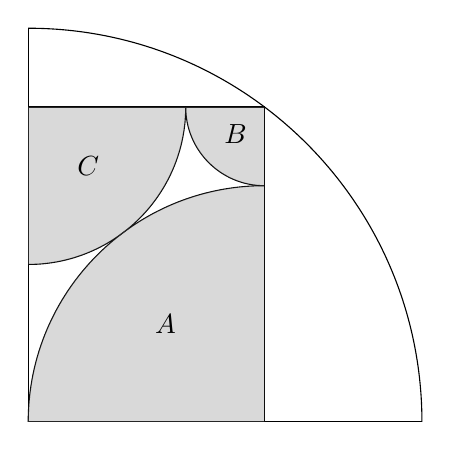
\begin{tikzpicture}
\draw (0,5) -- (0,0) -- (5,0);
% The coordinate for arcs is not the centre of their circle, it's the start of the arc
\draw (5,0) arc[start angle=0, end angle=90, radius=5];
\draw (3,0) -- (3,4) -- (0,4);
\draw (3,3) arc[start angle=90, end angle=180, radius=3];
\draw (3,3) arc[start angle=270, end angle=180, radius=1];
\draw (2,4) arc[start angle=0, end angle=-90, radius=2];
% Shade the quarter circle arcs
\fill[gray,opacity=0.3] (3,0) -- (3,3) arc[start angle=90, end angle=180, radius=3];
\fill[gray,opacity=0.3] (0,4) -- (2,4) arc[start angle=0, end angle=-90, radius=2];
\fill[gray,opacity=0.3] (3,4) -- (2,4) arc[start angle=180, end angle=270, radius=1];
% I'm just going to label the quarter circles manually
\coordinate[label=135:$A$] (A) at (2,1);
\coordinate[label=225:$B$] (B) at (2.9,3.9);
\coordinate[label=315:$C$] (C) at (0.5,3.5);
\end{tikzpicture}
\hspace{\fill}

To solve this problem, let's first define some lengths. We're going to declare the radius of $B$ to be 1, because it's the smallest length on the diagram. We'll also declare the radius of $A$ to be $x$. Thus, the radius of $C$ is $x - 1$.

\hspace{\fill}
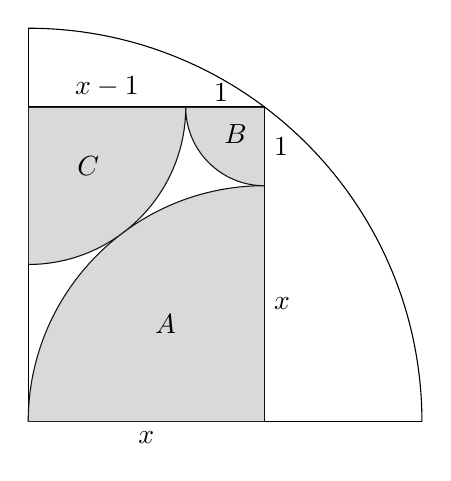
\begin{tikzpicture}
% This first bit is just the base diagram
\draw (0,5) -- (0,0) -- (5,0);
\draw (5,0) arc[start angle=0, end angle=90, radius=5];
\draw (3,0) -- (3,4) -- (0,4);
\draw (3,3) arc[start angle=90, end angle=180, radius=3];
\draw (3,3) arc[start angle=270, end angle=180, radius=1];
\draw (2,4) arc[start angle=0, end angle=-90, radius=2];
\fill[gray,opacity=0.3] (3,0) -- (3,3) arc[start angle=90, end angle=180, radius=3];
\fill[gray,opacity=0.3] (0,4) -- (2,4) arc[start angle=0, end angle=-90, radius=2];
\fill[gray,opacity=0.3] (3,4) -- (2,4) arc[start angle=180, end angle=270, radius=1];
\coordinate[label=135:$A$] (A) at (2,1);
\coordinate[label=225:$B$] (B) at (2.9,3.9);
\coordinate[label=315:$C$] (C) at (0.5,3.5);
% Then we label the declared new lengths
\coordinate[label=270:$x$] (x) at (1.5,0);
\coordinate[label=0:$x$] (x) at (3,1.5);
\coordinate[label=0:$1$] (1) at (3,3.5);
% This label's fiddly because it touches the circle if done normally
\coordinate[label=90:$1$] (1) at (2.45,3.94);
\coordinate[label=90:$x - 1$] (x-1) at (1,4);
\end{tikzpicture}
\hspace{\fill}

We're now going to draw a diagonal line across the rectangle. This line passes through the point where $A$ and $C$ kiss. This is because circles can only kiss on the line that passes through both their centres, and in this case, that line is the diagonal of this rectangle.

I'll remove the shading and labels to make things easier to see.

\hspace{\fill}
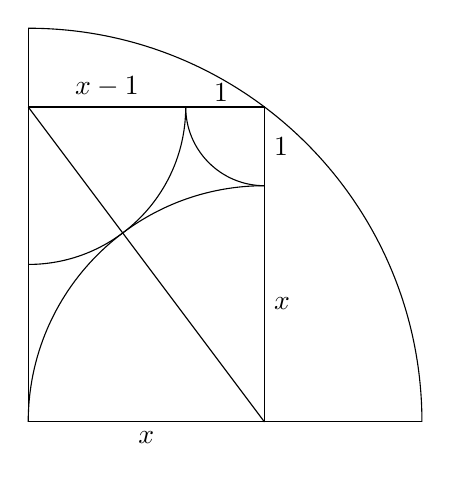
\begin{tikzpicture}
\draw (0,5) -- (0,0) -- (5,0);
\draw (5,0) arc[start angle=0, end angle=90, radius=5];
\draw (3,0) -- (3,4) -- (0,4);
\draw (3,3) arc[start angle=90, end angle=180, radius=3];
\draw (3,3) arc[start angle=270, end angle=180, radius=1];
\draw (2,4) arc[start angle=0, end angle=-90, radius=2];
\coordinate[label=270:$x$] (x) at (1.5,0);
\coordinate[label=0:$x$] (x) at (3,1.5);
\coordinate[label=0:$1$] (1) at (3,3.5);
\coordinate[label=90:$1$] (1) at (2.45,3.94);
\coordinate[label=90:$x - 1$] (x-1) at (1,4);
% This is the new line
\draw (0,4) -- (3,0);
\end{tikzpicture}
\hspace{\fill}

This line can be thought of as having two components. The radius of $A$, which is $x$, and the radius of $C$, which is $x - 1$. Thus, the length of this line is $x + x - 1 = 2x - 1$.

We can also see that this line is the hypotenuse of a right triangle with catheti $x$ and $x + 1$. Thus, by Pythagoras, we can say $(2x - 1)^2 = x^2 + (x + 1)^2$. Then, we can solve for $x$.
\begin{gather*}
4x^2 - 4x + 1 = x^2 + x^2 + 2x + 1\\
4x^2 - 4x + 1 = 2x^2 + 2x + 1\\
2x^2 - 6x = 0\\
2x(x - 3) = 0\\
x(x - 3) = 0
\end{gather*}
We can now see that $x$ is either equal to 0 or 3. $x$ equalling 0 doesn't make sense, so $x$ must equal 3.

Before labelling our diagram with concrete values, it is useful to see that changing the direction of this diagonal line through the rectangle doesn't change its length.

\hspace{\fill}
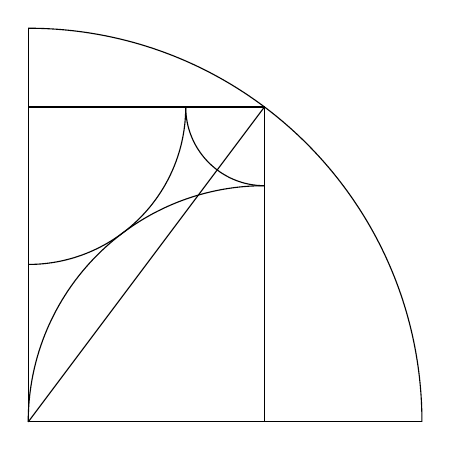
\begin{tikzpicture}
\draw (0,5) -- (0,0) -- (5,0);
\draw (5,0) arc[start angle=0, end angle=90, radius=5];
\draw (3,0) -- (3,4) -- (0,4);
\draw (3,3) arc[start angle=90, end angle=180, radius=3];
\draw (3,3) arc[start angle=270, end angle=180, radius=1];
\draw (2,4) arc[start angle=0, end angle=-90, radius=2];
% This is the new (backwards) line
\draw (3,4) -- (0,0);
\end{tikzpicture}
\hspace{\fill}

This line still has a length of $2x - 1$, and it's also the radius of the big quarter circle. Since we know that $x = 3$, we now know that the radius of the big circle is $2 \times 3 - 1 = 5$. We now have all the information we need to solve the problem.

\hspace{\fill}
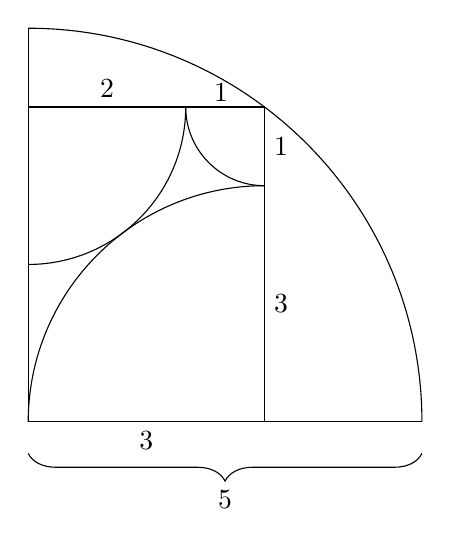
\begin{tikzpicture}
\draw (0,5) -- (0,0) -- (5,0);
\draw (5,0) arc[start angle=0, end angle=90, radius=5];
\draw (3,0) -- (3,4) -- (0,4);
\draw (3,3) arc[start angle=90, end angle=180, radius=3];
\draw (3,3) arc[start angle=270, end angle=180, radius=1];
\draw (2,4) arc[start angle=0, end angle=-90, radius=2];
\coordinate[label=270:$3$] (3) at (1.5,0);
\coordinate[label=0:$3$] (3) at (3,1.5);
\coordinate[label=0:$1$] (1) at (3,3.5);
\coordinate[label=90:$1$] (1) at (2.45,3.94);
\coordinate[label=90:$2$] (2) at (1,4);
% This is a brace for the radius of the big arc
\draw [decorate,decoration={brace,amplitude=10pt,mirror}] (0,-0.4) -- (5,-0.4);
\coordinate[label=270:$5$] (5) at (2.5,-0.75);
\end{tikzpicture}
\hspace{\fill}

First, we need the sum of the areas of the small quarter circles. This is
\begin{gather*}
\qpi \times 3^2 + \qpi \times 1^2 + \qpi \times 2^2\\
= \pif (9 + 1 + 4)\\
= \pif \times 14
\end{gather*}

I could simplify this, but we're going to cancel $\pif$.

The area of the big circle is $\qpi \times 5^2 = \pif \times 25$. Thus, the ratio between these areas is $$\frac{\cancel{\pif} \times 14}{\cancel{\pif} \times 25} = \frac{14}{25} = 56\%$$

\end{document}
